\newpage
\begin{song}{title={Chłopcy z Botany Bay}, music={Mietek Folk}, capo=3}
\begin{multicols}{2}
    \begin{verse}
        Już nad ^{h}Hornem ^{A}zapada ^{h}noc \\
        Wiatr na ^{h}żaglach ^{A}położył ^{D}się \\
        |: A tam ^{G}jeszcze ^{A}korsarze na ^*{D}Bota ^{A}ny ^{h}Bay | \\
        | Upy^{G}chają ^{A}zdobycze ^{h}swe :|
    \end{verse}
    \begin{verse}
        Jolly Roger na maszcie już śpi \\
        Jutro przyjdzie z Hiszpanem się bić \\
        A korsarze znużeni na Botany Bay \\
        Za zwycięstwo dziś będa swe pić
    \end{verse}
    \begin{verse}
        Śniady Clark puchar wznosi do ust \\
        "Bracia, toast! Niech idzie na dno!" \\
        Tylko Johnny nie pije, bo kilka mil stąd \\
        Otuliło złe morze go
    \end{verse}
    \begin{verse}
        Nie podnosi kielicha do ust \\
        Zawsze on tu najgłośniej się śmiał \\
        Mistrz fechtunku z Florencji ugodził go \\
        Już nie będzie za szoty się brał
    \end{verse}
    \begin{verse}
        W starym porcie zapłacze Margot \\
        Jej kochany nie wróci już \\
        Za dezercję do panny na kei w Brisbane \\
        Oddać musiał swą głowę pod nóż
    \end{verse}
    \begin{verse}
        Tak niewielu zostało dziś ich \\
        Resztę zabrał Neptun pod dach \\
        Choć na ustach wciąż uśmiech, to w sercach lód \\
        W kuflu miesza się rum i strach
    \end{verse}
    \begin{verse}
        To ostatni chyba już rejs \\
        Cios sztyletem lub kula w pierś \\
        Bóg na szkuner w niebiosach zabierze ich \\
        Wszystkich chłopców z Botany Bay
    \end{verse}
    \begin{verse}
        Już nad Hornem zapada noc \\
        Wiatr na żaglach położył się \\
        A tam jeszcze korsarze na Botany Bay \\
        Upychają zdobycze swe
    \end{verse}
\end{multicols}
\begin{center}
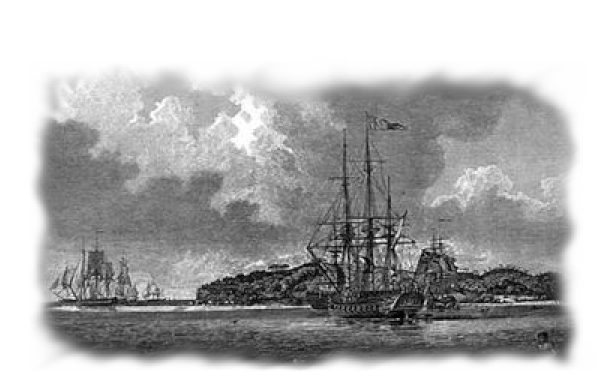
\includegraphics[width=0.7\textwidth]{images/botany_bay.png}  
\end{center}
\end{song}

